\chapter{Lyntax: Proposal} \label{lyntax_proposal}

The main purpose of this proposal is the definition of a \textsc{DSL} that allows the specification of all different kinds of sentences (done by the linguistic teacher), and afterwards, the possibility of the student to test his own sentences and check if they are written accordingly to the rules also previously specified by the linguistic teacher. One obstacle that was encountered was how to extract the lexical part of the sentence, and in what way would each component be classified. In fact, this task is quite subjective, as different components may have various definitions in one context. % for example: (...). % Introduzir exemplo da professora!!!! 
Having known this, the decision was made that the student would beforehand identify the lexical part of the sentence.
% FALAR DO QUE VOU FAZER DE DIFERENTE (DICA DO LÁZARO!)


\section{System Architecture}
In order to specify all kinds of sentences/rules possible, the idea of creating a ``meta-language'' emerged. This ``meta-language'' will be used by the teacher to specify the rules for sentence construction. 
These rules will be written (in a single file) according to the following structure, that is divided into three main categories:

\begin{enumerate}
    \item \textbf{STRUCTURE} - the block where the teacher will write how is the sentence supposed to be written, and what components will it have.
    
    \item \textbf{ERRORS/RULES} - list of conditions that the teacher could write in order to be analysed afterwards, for example, certain values for different attributes. 
In the case of using ERRORS, if the conditions are matched, an error will appear. 
On the other hand, using RULES, the conditions need to be matched in order to have a valid input.
    
    \item \textbf{INPUT} - this block corresponds to the ``parsing'' of the sentence (the lexical part) that the student wants to test. This will be written by the student and then automatically joined with the teachers information.
\end{enumerate}

% Imagem da arquitetura do sistema.
\begin{figure}[h]
    \centering
    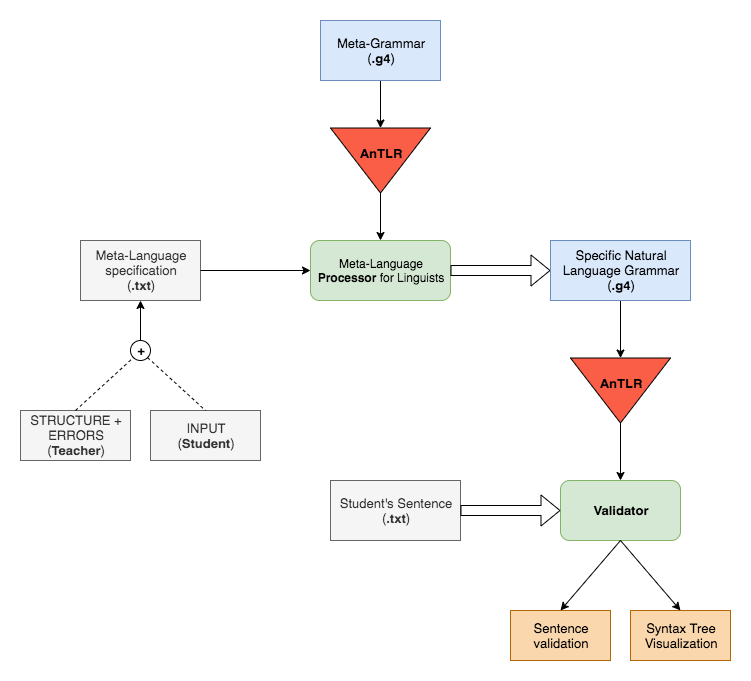
\includegraphics[width=12cm]{images/msc_system_architecture.png}
    \caption{System architecture.}
    \label{fig:system_architecture}
\end{figure}

This file will then be processed by an \textsc{ANTLR} processor that will work on the information that was written, and then generate a grammar (also specified in \textsc{ANTLR}). 
This grammar corresponds to the translation of the ``meta-language'' into \textsc{ANTLR} instructions. 
Afterwards, the generated grammar will be used to create a validator of sentences, where the student can write his sentence/sentences and obtain results.
A new processor will be generated for each sentence the student wants to test.
The results would be the validation of the given sentence/sentences and a tree for a better visualization of the input structure.


\section{Meta-Language}
As it was stated in the beginning of this document, the main goal was to create a \textsc{DSL} that should be easy to learn and to rapidly understand and grasp. With this in mind, the structure mencioned before on the first section
of this chapter was followed: Three main parts, where two of them would be constructed by the teacher, and the third one was intended to be written by the student and later concatenated in a single file.

\subsection{Domain Specific Meta-Grammar}
The main intention of this language is to preprocess the information written by the teacher + student and then generate a validator for a particular structure. With simplicity in mind, a first version of the \textsc{DSL} was created, and it will be explained next.

\begin{center}
\begin{minipage}{8cm}
\begin{lstlisting}[language=java, basicstyle=\small, label={lst:processor_prod}, caption=Processor production]
processor : structure errors input
;
\end{lstlisting}
\end{minipage}
\end{center}

Firstly, the teacher specification will be discussed - meaning the \textbf{structure} and \textbf{errors} blocks.
The \textbf{structure} block is divided into \textbf{parts}, or main parts. These main parts correspond to the main components of the sentence. Each of these parts have an \textbf{element} within, containing the information about a certain component.

\begin{center}
\begin{minipage}{14cm}
\begin{lstlisting}[language=java, basicstyle=\small, label={lst:dsl_struct_prod}, caption=DSL structure/part/element productions]
structure : 'STRUCTURE:' (part)+ ;

part : 'part' '[' element ']' ;

element : '(' WORD ( '|' WORD )* ( ',' attributes )? ( ',' subparts )? ')' 
    ('?')? ;
\end{lstlisting}
\end{minipage}
\end{center}

The \textbf{element} is composed by the name of the component, a possible set of \textbf{attributes} and possible \textbf{subparts}.

\begin{center}
\begin{minipage}{13cm}
\begin{lstlisting}[language=java, basicstyle=\small, label={lst:dsl_attrs_prod}, caption=DSL attributes/subparts productions]
attributes : 'attributes' '{' WORD ( ',' WORD )* '}'
;

subparts : 'subparts' '[' element ( ',' element ) ']'
;
\end{lstlisting}
\end{minipage}
\end{center}

The \textbf{subparts} production intends to be the path for ``injecting'' more elements inside a single component. One component may be composed by several other components. As shown in the example above, the \textbf{subparts} production is a list of one or more elements.

Secondly, the teacher can define a list of restrictions to be applied to each attribute defined in the previous structure. A sentence will be valid if it follows the specified structure and if it obeys to the specified conditions.

\begin{center}
\begin{minipage}{12cm}
\begin{lstlisting}[language=java, basicstyle=\small, label={lst:dsl_errors_prod}, caption=DSL errors/expression productions]
errors : ('RULES'|'ERRORS') ':' ( condition ';' )+
;

condition : assignment ( ('AND'|'OR') assignment )*
;
\end{lstlisting}
\end{minipage}
\end{center}

The \textbf{errors} production will have two meanings: if the keyword use is 'RULES', then the conditions defined by the teacher need to be checked in order for a sentence to be correct; on the other hand, if the keyword is 'ERRORS', then if the conditions are matched, the sentence is not considered correct within that structure.
The \textbf{condition} production is composed by a set of assignments that can be joined using the logical operators 'AND' and 'OR'. 
Each condition intends to create logical evaluations for the various attributes defined.
Conditions are composed by assignments, which are composed by expressions.

\begin{center}
\begin{minipage}{10cm}
\begin{lstlisting}[language=java, basicstyle=\small, label={lst:dsl_cond_prod}, caption=DSL condition production]
assignment 
    : expression ('='|'!=') expression
    | expression ('='!'!=') '"' WORD '"'
;

expression : WORD ( '.' WORD )* '->' WORD 
;
\end{lstlisting}
\end{minipage}
\end{center}

The \textbf{assignment} production assigns an \textbf{expression}, which is composed by the path to a certain attribute, to a value or to other expression. 
If, for instance, the teacher says that an attribute is equal to some value, then the student can not use other value to that attribute - this would result in an error.

Thirdly, and finally, the \textbf{input} block, which corresponds to the students section. This was treated has a different and separate \textsc{DSL}, as its main purpose was to identify the lexical parts of the sentence written 
by the student, allowing for a correct and non-subjective parsing of each word in the sentence.

\begin{center}
\begin{minipage}{8cm}
\begin{lstlisting}[language=java, basicstyle=\small, label={lst:dsl_input_prod}, caption=DSL input production]
input : 'INPUT:' phrase 
;

phrase : ( '-' parts )+
;
\end{lstlisting}
\end{minipage}
\end{center}

The sketch starts within a section named \textbf{phrase}, which corresponds to one sentence in particular. 
This production is composed by one or more \textbf{parts}, each of them holding various \textbf{blocks}, where all the information is stored. 
Inside, the name of the components and their required attributes must be specified. 
It is also important to notice that a correct path must be specified by the student. 
If the student specifies a component that is not declared in the structure defined previously by the teacher, then an error should be thrown.

\begin{center}
\begin{minipage}{10cm}
\begin{lstlisting}[language=java, basicstyle=\small, label={lst:dsl_parts_prod}, caption=DSL parts/component/content productions]
parts : '(' block ( ',' block )* ')'
;

block : WORD content
;

content : (slice)? (attrs)? (parts)?
;
\end{lstlisting}
\end{minipage}
\end{center}

The student can specify the \textbf{slice} of the sentence that corresponds to the component that is being declared, and a set of attributes (\textbf{attrs}) that composes said component. Furthermore, it is possible to continue to define more \textbf{parts} within one part, just like the teacher's \textsc{DSL} \textbf{subparts}.

\begin{center}
\begin{minipage}{11cm}
\begin{lstlisting}[language=java, basicstyle=\small, label={lst:dsl_slice_prod}, caption=DSL slice/attrs/evaluations/eval productions]
slice : ':' '``' (WORD)+ '"'
;

attrs : '[' evaluations ']'
;

evaluations : eval ( ',' eval )*
;

eval : WORD '=' '``' WORD '"'
;
\end{lstlisting}
\end{minipage}
\end{center}

Inside the \textbf{slice} production, a list of words can be written. These are the words that will then be used to build the lexical part of the generated grammar. Also, when specifying attributes, the student must assign a value for each attribute that will then be used to validate each component of the sentence.

For a better understanding of the three main categories (structure, errors and input), bellow there is an example that is based on the first case study, and shows what the specification of the teacher should look like.

\begin{center}
\begin{minipage}{13cm}
\begin{lstlisting}[language=java, basicstyle=\tiny, label={lst:metaStruct}, caption=Example of a possible sentence structure]
STRUCTURE:
	part[(
        Sujeito, 
        attributes{tipo}, 
        subparts[
            (Determinante)?, 
            (Nome)
        ]
	)]
    
	part[(
        Predicado,
        subparts[
            (Verbo, attributes{tipo}),
            (Complemento_Direto, subparts[(Determinante)?, (Nome)]),
        ]
	)]

ERRORS:
    Sujeito->tipo = ``animado" AND Predicado.Verbo->tipo = ``inanimado";
    Sujeito->tipo = ``inanimado" AND Predicado.Verbo->tipo = ``animado";
\end{lstlisting}
\end{minipage}
\end{center}

In the case of the student, this is the specification that should be used and one of the many examples that fit into the defined structured.

\begin{center}
\begin{minipage}{13cm}
\begin{lstlisting}[language=java, basicstyle=\tiny, label={lst:metaInput}, caption=Example of the students parsing]
INPUT:
    - (Sujeito: ``O Carlos" [tipo = ``animado"]
        (Determinante: ``O", Nome: ``Carlos"))
    - (Predicado: ``teme a sinceridade" 
        (Verbo: ``teme" [tipo = ``animado"], Complemento_Direto: ``a sinceridade" 
            (Determinante: ``a", Nome: ``sinceridade")))
\end{lstlisting}
\end{minipage}
\end{center}


\section{Chapter Summary}

In this chapter, it was discussed the different phases of the proposed system architecture and what the output of a system like this should be.
The principle is to create a new Domain Specific (Meta) Language that allows for the specification of sentence structures as well as proper input.
Within this system, a processor for this Meta-Language is created by using \textsc{ANTLR},
which evaluates the specification written and is tasked with the generation of a specific natural language grammar.
Combining the newly generated grammar with \textsc{ANTLR}, the result is a student's sentence validator
that when given a sentence as input, performs all the necessary validations and, if correct, presents the user the respective syntax tree.

\textbf{Lyntax}, the word that combines the terms ``Linguistics" and ``Syntax", was the name chosen for a system that combines both the meta-language processor and
the user interface that makes use of such processor.
The implementation of this system will be discussed in the next section.
